

% Auriga theme
% https://github.com/anishathalye/auriga

\documentclass[14pt,aspectratio=169]{beamer}
\usepackage{pgfpages}
\usepackage{fancyvrb}
\usepackage{booktabs,dcolumn}
\usepackage{tikz}
\usetikzlibrary{arrows.meta, positioning, quotes}
\usepackage{pgfplots}

% \ifnotes
% \setbeamertemplate{note page}[plain]
% \setbeameroption{show notes on second screen=right}
% \fi

\usetheme{auriga}
\usecolortheme{auriga}

% define some colors for a consistent theme across slides
\definecolor{red}{RGB}{181, 23, 0}
\definecolor{blue}{RGB}{0, 118, 186}
\definecolor{gray}{RGB}{146, 146, 146}

\title{Historia Económica Argentina}

\author{\underline{Sebastián Freille} \inst{1}}

\institute[shortinst]{\inst{1} IEF-UNC \\ UCC}
\date{}

\AtBeginSection[]{
    \begin{frame}
    \vfill
    \centering
    \begin{beamercolorbox}[sep=8pt,center,shadow=true,rounded=true]{title}
        \usebeamerfont{title}\insertsectionhead\par%
    \end{beamercolorbox}
    \vfill
    \end{frame}
}



\AtBeginSubsection[]{
    \begin{frame}
    \vfill
    \centering
    \begin{beamercolorbox}[sep=6pt,center,shadow=true,rounded=true]{title}
        \usebeamerfont{title}\insertsubsectionhead\par%
    \end{beamercolorbox}
    \vfill
    \end{frame}
}


\AtBeginSubsubsection[]{
    \begin{frame}
    \vfill
    \centering
    \begin{beamercolorbox}[sep=4pt,center,shadow=true,rounded=true]{title}
        \usebeamerfont{title}\insertsubsubsectionhead\par%
    \end{beamercolorbox}
    \vfill
    \end{frame}
}


\begin{document}

{
  % rather than use the frame options [noframenumbering,plain], we make the
  % color match, so that the indicated page numbers match PDF page numbers
  \setbeamercolor{page number in head/foot}{fg=background canvas.bg}
  \begin{frame}
    \titlepage
  \end{frame}
}


\section{Cap 5. La década de expansión}

\begin{frame}\frametitle{Un nuevo intento de democracia}
                 \begin{itemize}\itemsep 5pt \medskip
                 \item La elección de 1963 fue restringida
                   --candidatos peronistas proscriptos. Nuevamente la
                   explicación el profundo anti-peronismo del ala
                   militar
                   \item Pero la influencia de Perón era importante
                     --20\% de votos en blanco fue la segunda minoría
                     \item Illia pertenecía a un radicalismo diferente
                       al de Frondizi (linea Yrigoyenista)
                   \end{itemize}
               \end{frame}


               \begin{frame}\frametitle{Un nuevo intento de democracia
                 (cont.)}
                 \begin{itemize}\itemsep 5pt \medskip
                 \item Illia tuvo un posición difícil --tanto el
                   peronismo (sindicalismo) como el ``partido militar'' condicionaban
                   la autoridad del presidente
                   \item La relación entre el gobierno y el
                     sindicalismo (CGT) fue
                     complicada --toma de fábricas, paros generales
                     \item El frente militar fue benigno al principio
                       pero luego radicalizó el discurso en pocos años
                       --convivencia dificultada por la posición ante
                       el regreso y ``habilitación'' del peronismo
                   \end{itemize}
               \end{frame}


                \begin{frame}\frametitle{Un nuevo intento de democracia
                 (cont.)}
                 \begin{itemize}\itemsep 5pt \medskip
                 \item El fantasma de un nuevo golpe cívico-militar
                   siempre sobrevoló la presidencia de Illia --medios
                   de comunicación sumaban tensión.
                   \item Hacia mediados de 1966, la tensión era
                     creciente y a finales de junio Illia (UCRP) es
                     derrocado.
                     \item Los jefes de las tres fuerzas militares
                       declararon el inicio de la Revolución Argentina
                       y Juan Carlos Onganía asume el poder. 
                   \end{itemize}
               \end{frame}

               


                \begin{frame}\frametitle{La economía de \textit{stop
                      and go}}
                 \begin{itemize}\itemsep 5pt \medskip
                 \item El contexto económico en que asume Illia era de
                   recesión prolongada (2 años) --desempleo en aumento
                   y salario real disminuido
                   \item Un tema central era la iliquidez y escasez de
                     crédito $\longrightarrow$ corte abrupto de K
                     exterior más política monetaria ortodoxa
                     \item Dadas las cosas, el objetivo prioritario de
                       Illia fue la reactivación económica --desafío
                       era superar definitivamente el esquema de
                       \textit{stop and go} que aquejaba a la economía
                       desde hacía más de 15 años --aumento de PBI pc
                       entre 1948-63 sólo de 4\% (promedio mundial del 50\%)
                   \end{itemize}
               \end{frame}

               
          
 
  \begin{frame}\frametitle{La economía de \textit{stop and go} (cont.)}
\begin{figure}[hxtbp]\vspace{0cm}
  \centering
  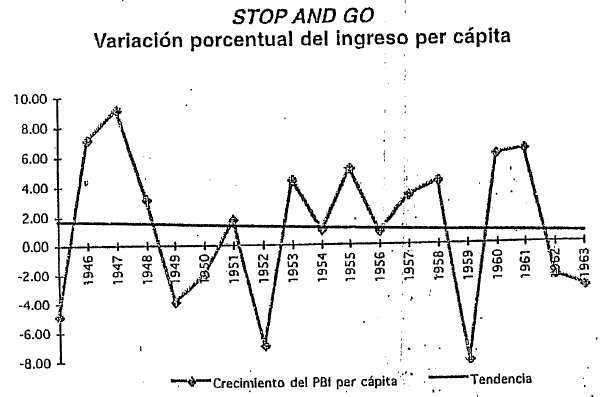
\includegraphics[scale=0.7]{uni5_illia01}
   \label{fig:uni1_01}
\end{figure} 
  \end{frame}


 \begin{frame}\frametitle{La economía de \textit{stop and go} (cont.)}
                 \begin{itemize}\itemsep 5pt \medskip
                 \item Condiciones de \textit{stop and go} una mezcla
                   de decisiones forzadas (década del 30) y voluntarias
                   (década del 40) $\longrightarrow$ extrema
                   vulnerabilidad exterior
                   \item La ISI se había completado para muchas ramas
                     industriales pero había fuerte dependencia
                     exterior en provisión de insumos,
                     maquinarias y equipo
                     \item Se necesitaban divisas para poder $M$ estos
                       bienes y las divisas dependían de lo que el
                       país pudiera $X$ --sesgo anti-exportador era un
                       gran problema
                   \end{itemize}
               \end{frame}

  \begin{frame}\frametitle{La economía de \textit{stop and go} (cont.)}
                 \begin{itemize}\itemsep 5pt \medskip
                 \item Ciclo de \textit{stop and go} aparecería
                   cada vez que las necesidades de
                   divisas para M superaran a las que podían generarse
                   por X --devaluación era la salida frecuente
                 \item Pero la devaluación tiene varios efectos:
                   \begin{itemize}\itemsep 5pt \medskip
                   \item Estimular X y desestimular M
                     \item Disminuir consumo privado tanto de $T$ como
                       de $NT$ dada la caída de
                       salario real --esto era particularmente
                       cierto en Argentina. 
                     \end{itemize}
                     \item La devaluación
                       generalmente venía acompañada de cierta
                       recesión --disminuía ``M'' y se revertía
                       déficit
                       \item Aumento de salario nominal gradual volvía
                         a estimular la económía al tiempo que
                         aumentaba costos domésticos. 
                   \end{itemize}
               \end{frame}


\begin{frame}\frametitle{La economía de \textit{stop and go} (cont.)}
  \begin{block}{Retardando el \textit{stop and go}}
En condiciones excepcionales --flujo sostenido de K- podía sostenerse
el crecimiento y fundamentalmente alterarse la estructura
productiva. Frondizi había sido un experimento a gran escala en esa
dirección: capitalizar el país por la vía de préstamos/inversiones
extranjeras. La recesión de 1962/63 (al igual que la de 1952 y 1959)
--causada por una creciente escasez de divisas causó el cuello de
botella y un nuevo ``stop''. 
    \end{block}
               \end{frame}
               
\section{El gobierno de Illia}


                \begin{frame}\frametitle{El gobierno de Illia}
                 \begin{itemize}\itemsep 5pt \medskip
                 \item Las primeras medidas apuntar a estimular la
                   demanda en el corto plazo: expansión fiscal y
                   emisión monetaria para estimular liquidez y crédito
                   \item Se congelaron tarifas de empresas de
                     servicios públicos $\longrightarrow$ para mejorar
                     salario real
                     \item Se sancionó la Ley de Salario Mínimo, Vital
                       y Móvil (1964) que llega hasta nuestros días
                       \item Crecimiento de salario nominal por encima
                         de inflación --aumento 10\% en términos reales
                   \end{itemize}
               \end{frame}



                \begin{frame}\frametitle{El gobierno de Illia (cont.)}
                 \begin{itemize}\itemsep 5pt \medskip
                 \item Para evitar un empeoramiento de las cuentas
                   externas se optó por renegociar deuda con países
                   acreedores (1965)
                   \item Medidas puntuales: crédito facilitado a
                     industrias intensivas en insumos nacionales,
                     suspensión de facilidades (fciamiento) a M
                     \item Política cambiaria fue adecuada a las
                       necesidades $\longrightarrow$ ni TCFi ni
                       TCFl sino \textit{crawling peg}
                       \item Hubo nueve devaluaciones pero no fueron
                         bruscas sino para ajustar a inflación interna
                   \end{itemize}
               \end{frame}


               \begin{frame}\frametitle{El gobierno de Illia (cont.)}
                 \begin{itemize}\itemsep 5pt \medskip
                 \item La estrategia \textit{crawling peg} garantiza
                   poder de compra el tipo de cambio efectivo de los
                   exportadores (gran problema)
                   \item Las X que habían estado estancadas durante
                     los últimos 35 años --en 1961 Argentina había
                     exportado \textit{menos} dólares en 1928!-, ven un crecimiento muy
                     promisorio
                     \item No todo fue mérito de la política cambiaria
                       sino que también ayudaron los altos precios
                       internacionales de 1964-65 y los factores climáticos
                   \end{itemize}
               \end{frame}
               


  \begin{frame}\frametitle{El gobierno de Illia (cont.)}
\begin{figure}[hxtbp]\vspace{0cm}
  \centering
  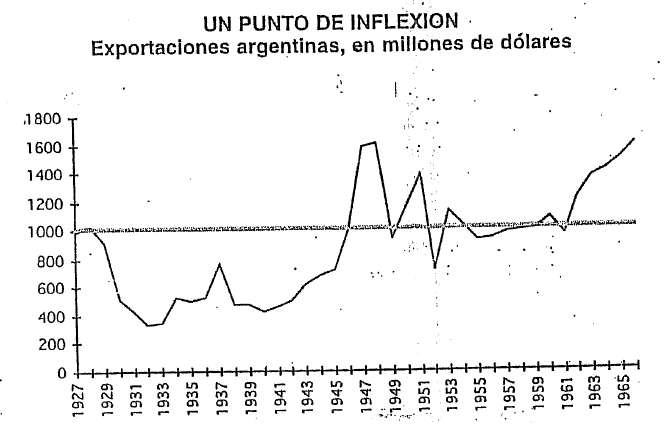
\includegraphics[scale=0.7]{uni5_illia02}
   \label{fig:uni1_01}
\end{figure} 
  \end{frame}




  
               \begin{frame}\frametitle{El gobierno de Illia (cont.)}
                 \begin{itemize}\itemsep 5pt \medskip
                 \item Fue tal el aumento de las cantidades exportadas
                   (y producidas) que aumentó la participación de
                   actividades primarias en el PBI.
                   \item Este aumento de las X representó un punto de
                     inflexión en el frente externo --una barrea (1000
                     millónes de dólares) que había resultado de
                     dificil superación anteriormente
                     \item Producción agropecuaria más alta que el
                       promedio histórico --60\% de aumento en
                       cereales, 20\% aumento en ganado entre 1963 y 1965
                   \end{itemize}
                 \end{frame}


                   \begin{frame}\frametitle{El gobierno de Illia (cont.)}
                 \begin{itemize}\itemsep 5pt \medskip
                 \item Una de las excepciones al manejo moderado de la
                   política económica de Illia fue la cuestión del
                   petróleo $\longrightarrow$ anulación de contratos
                   con firmas extranjeras
                   \item Medida coherente con ideología pero problema
                     en términos de credibilidad internacional
                     $\longrightarrow$ más aún, se detuvo bruscamente el
                     crecimiento del sector
                     \item Reaparece una fuente de drenaje de divisas
                       (M de petróleo)
                   \end{itemize}
               \end{frame}



                \begin{frame}\frametitle{El gobierno de Illia (cont.)}
                 \begin{itemize}\itemsep 5pt \medskip
                 \item A pesar de las críticas al plan del gobierno,
                   la estrategia de reactivación (PF y PM expansivas)
                   sumada a una política cambiaria sensata, los años
                   1964 y 1965 vieron un crecimiento promedio del 10\%
                   \item Además, la inversión como porcentaje del PBI
                     estuvo cerca del 20\%
                     \item El desempleo bajó de 8.8\% a 4.6\%. El
                       saldo comercial entre 1963-66 fue casi el de un
                       año total de X
                       \item No había indicios de problemas externos
                   \end{itemize}
               \end{frame}



 \begin{frame}\frametitle{El gobierno de Illia (cont.)}
\begin{figure}[hxtbp]\vspace{0cm}
  \centering
  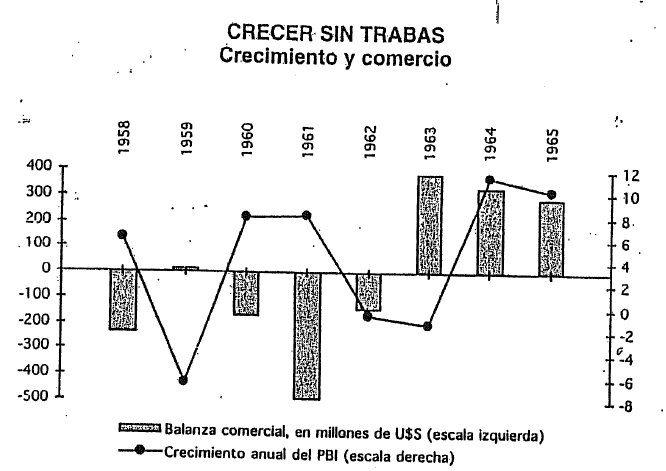
\includegraphics[scale=0.7]{uni5_illia03}
   \label{fig:uni1_01}
\end{figure} 
  \end{frame}


                \begin{frame}\frametitle{El gobierno de Illia (cont.)}
                 \begin{itemize}\itemsep 5pt \medskip
                 \item Sin embargo, había una doble sensación a
                   principios de 1966 $\longrightarrow$ crisis
                   económica y política en ciernes
                   \item Se aludía al deterioro de la BP para
                     anticipar la recesión --PBI aumentó sólo un 1\%
                     pero no hubo crisis de BP [temor de nuevo
                     \textit{stop and go} se alejaba]
                     \item En el frente político, sin embargo, el fin
                       de Illia estaba cerca luego de mucho desgaste
                    en las relaciones políticas. 
                   \end{itemize}
               \end{frame}



         \section{La Revolución Argentina: 1966-73}
      


             \begin{frame}\frametitle{La Revolución Argentina}
                 \begin{itemize}\itemsep 5pt \medskip
                 \item La caída forzada de Illia no puede atribuirse a
                   razones de índole económica
                   \item La llegada de Onganía fue de algún modo la
                     culminación de un proceso de modernización de las
                     fuerzas de las fuerzas armadas
                     \item El golpe tuvo objetivos ambiciosos
                       $\longrightarrow$ se buscaba el desarrollo
                       económico para luego normalización
                       institucional
                       \item Diferentes tiempos $\longrightarrow$ 1)
                         económico; 2) social; 3) político
                   \end{itemize}
               \end{frame}


  \begin{frame}\frametitle{La Revolución Argentina (cont.)}
                 \begin{itemize}\itemsep 5pt \medskip
                 \item En medio año de gobierno, la imagen de Onganía
                   habia caido por razones políticas fundamentalmente
                   (noche de bastones largos, mayo Francés, Cordobazo)
                   \item De 1969 a 1973, Argentina tuvo una creciente
                     conflictividad política, social y sindical (ERP,
                     Montoneros) y los militares reconocían que era
                     necesaria un regreso a la institucionalidad
                     política
                     \item Todo estaba dado para el regreso de Perón a
                       la vida política luego de 17 años en el exilio
                   \end{itemize}
               \end{frame}


\begin{frame}\frametitle{La Revolución Argentina (cont.)}
  \begin{itemize}\itemsep 5pt \medskip
    \item Puede dividirse en tres fases/etapas el período de la
      Revolución Argentina:
      \begin{itemize}\itemsep 5pt \medskip
      \item Preparativos (1966-67)
      \item Estabilización (1967-70) con el plan Krieger Vasena
        \item Declinación (1970-73) con devaluaciones, estimulos al
          crecimiento e inflación
        \end{itemize}
      \item Hacia finales de la Revolución Argentina, el ``tiempo
        político'' había llegado pero sin cumplir adecuadamente la
        pretensión de desarrollo económico
        \end{itemize}
               \end{frame}

               
\begin{frame}\frametitle{La Revolución Argentina (cont.)}
                 \begin{itemize}\itemsep 5pt \medskip
                 \item A pesar de toda la inestabilidad política
                   durante 1963 a 1973, Argentina contó con una
                   economía mundial floreciente
                   \item Entre 1950 y 1973, PBI per capita mundial creció
                     2.9\% anual --entre 1963-73 al 3.3\%
                     \item Fue uno de los mayores periodos de
                       crecimiento del siglo XX --en gran parte
                       impulsado por el aumento del comercio mundial
                       de ByS y de flujos de capital [acuerdo Bretton-Woods]
                   \end{itemize}
               \end{frame}




 \begin{frame}\frametitle{La Revolución Argentina (cont.)}
\begin{figure}[hxtbp]\vspace{0cm}
  \centering
  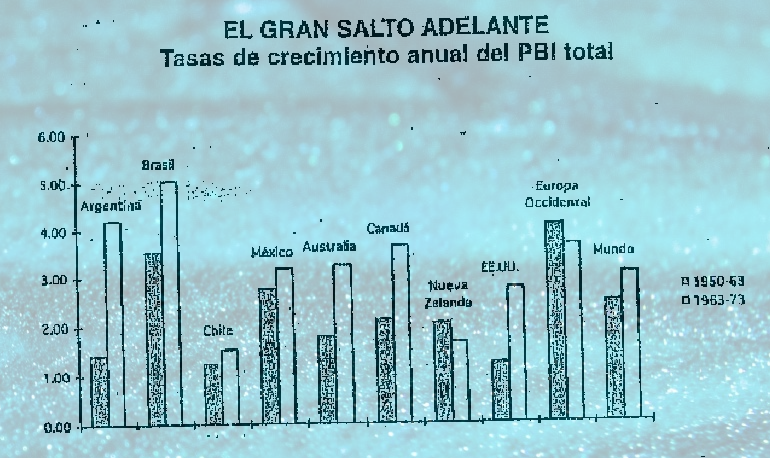
\includegraphics[scale=0.7]{uni5_onga02}
   \label{fig:uni1_01}
\end{figure} 
  \end{frame}



  

 \begin{frame}\frametitle{La Revolución Argentina (cont.)}
\begin{figure}[hxtbp]\vspace{0cm}
  \centering
  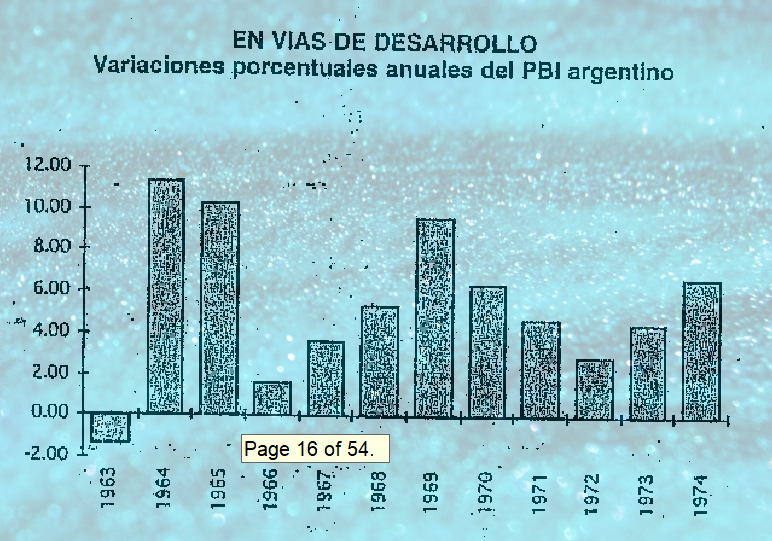
\includegraphics[scale=0.7]{uni5_onga01}
   \label{fig:uni1_01}
\end{figure} 
  \end{frame}

\begin{frame}\frametitle{La Revolución Argentina (cont.)}
                 \begin{itemize}\itemsep 5pt \medskip
                 \item Resulta extraño considerar a la década de los
                   60s como parte de las décadas perdidas
                   $\longrightarrow$ hubo algunas revisiones
                   estadísticas pero también era parte del clima
                   intelectual de época
                   \item La \textit{teoría de la dependencia}
                     --economías periféricas sujetas a las necesidades
                     de las economías centrales- influyó negativamente
                     en la percepción de crecimiento economico
                     \end{itemize}
               \end{frame}



\begin{frame}\frametitle{La Revolución Argentina (cont.)}
                 \begin{itemize}\itemsep 5pt \medskip
                 \item ¿Qué factores estuvieron detrás del gran
                   crecimiento económico de la década?
                   \begin{itemize}\itemsep 5pt \medskip
                   \item Avances en productividad rural
                     $\longrightarrow$ modernización del agro
                     \item Recuperación de la inversión de tiempos de Frondizi
                     \end{itemize}
                     \item En este sentido, el fuerte crecimiento de
                       esta década fue producto de una conjunción de
                       factores externos, transformaciones de periodos
                       anteriores y políticas económicas acertadas
                   \end{itemize}
               \end{frame}
               

\begin{frame}\frametitle{La Revolución Argentina (cont.)}
                 \begin{itemize}\itemsep 5pt \medskip
                 \item Importante impulso de la agricultura (no
                   tanto ganadería) --aumento de casi 50\% de
                   producción de cultivos (trigo, maiz, soja, sorgo y
                   girasol)
                   \item Gran responsable de esto fue la
                     ``mecanización del agro'' (tractores, tanto en
                     cantidad como calidad); además, uso de semillas
                     mejoradas y variedades híbridas
                     \item Tipo de cambio efectivo de agricultura sin
                       grandes oscilaciones bruscas
                   \end{itemize}
               \end{frame}





 \begin{frame}\frametitle{La Revolución Argentina (cont.)}
\begin{figure}[hxtbp]\vspace{0cm}
  \centering
  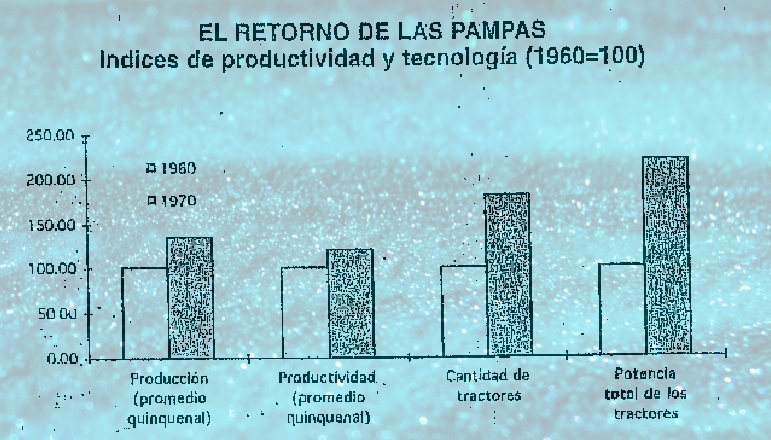
\includegraphics[scale=0.7]{uni5_ong03}
   \label{fig:uni1_01}
\end{figure} 
  \end{frame}
               

               \begin{frame}\frametitle{La Revolución Argentina (cont.)}
                 \begin{itemize}\itemsep 5pt \medskip
                 \item Esta política más predecible (buenos precios
                   externos mas uso discrecional de retenciones) dio
                   un gran impulso a la balanza comercial y de pagos
                   de Argentina
                   \item Diez de once años entre 1963-73 cerraron con
                     superavit --excedente se explica más por aumento
                     de X que por disminución de M (mejora tardía se
                     debe a fenomenal aumento de TIE en 1973)
                     \item Importante aumento de exportaciones no
                       tradicionales (industriales) como proporción
                       del total exportado, de 10\% a 20\%
                   \end{itemize}
               \end{frame}
               


 \begin{frame}\frametitle{La Revolución Argentina (cont.)}
\begin{figure}[hxtbp]\vspace{0cm}
  \centering
  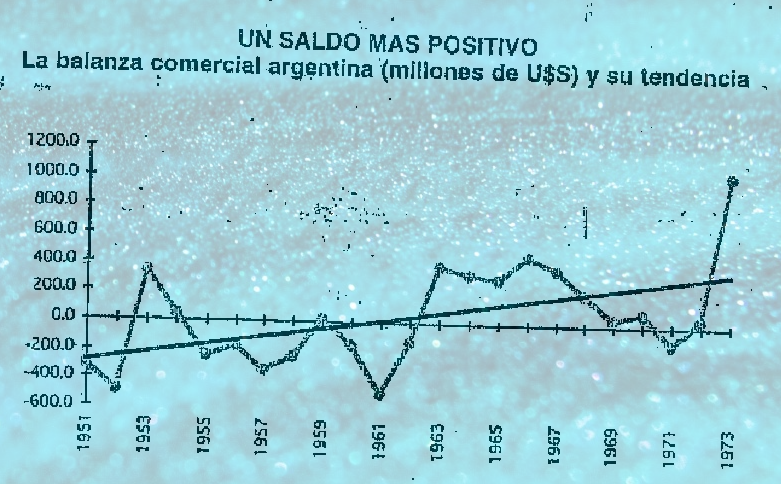
\includegraphics[scale=0.7]{uni5_onga04}
   \label{fig:uni1_01}
\end{figure} 
  \end{frame}



               \begin{frame}\frametitle{La Revolución Argentina (cont.)}
                 \begin{itemize}\itemsep 5pt \medskip
                 \item En este sentido, durante este período hubo
                   algún intento de fomentar las exportaciones
                   industriales a través algunas medidas no ortodoxas
                   (tipos de cambio múltiples)
                 \item También hubo políticas diferenciales a las X
                   tradicionales y no tradicionales (retenciones a las
                   primeras y reembolsos a las segundas)
                   \item Así y todo, la performace de exportaciones
                     industriales en su conjunto fue dispar y mediocre
                     en relación a la brasileña, por ejemplo.
                     \item Casi toda la producción industrial
                       destinada la mercado interno
                 \end{itemize}
               \end{frame}
               

    \begin{frame}\frametitle{La Revolución Argentina (cont.)}
                 \begin{itemize}\itemsep 5pt \medskip
                 \item Nuevamente se puso en discusión el tipo de
                   industrias que debían favorecerse y estimularse
                   desde la política económica
                   \item Las propuestas más audaces tenian que ver con
                     promover un patrón de industrias naturales, en el
                     sentido de aquellas con ventajas comparativas
                     \item Debian concentrarse en aquellas que
                       requerían factores de produción
                       (capital/trabajo) similares a las existentes en Argentina
                 \end{itemize}
               \end{frame}
               
  
               
\end{document}

%%% Local Variables:
%%% TeX-engine: lualatex
%%% TeX-master: t
%%% End: